\section{Problem Pinning}

We can use DR plans to help in solving questions in designs for graphene and silica bilayers (\todo{Add Citation}). Specifically, we will look into the problem when you have a monolayer and it is underconstrained. To make this thing isostatic, there are a few methods we can apply.

\begin{figure}\centering
    \includegraphics[width=0.5\linewidth]{img/Silica}
    \caption{Example of 1 layer of a Silica Oxygen glassy structure. This can be thought of as a multi-triangle-pin qusec where the Silicon atoms are the triangles and the Oxygen atoms are the pins.}
\end{figure}


\begin{itemize}
    \item Pin together 2 underconstrained monolayers in such a way that the resulting bilayer becomes isostatic.
    \item Pin the boundary in such a way that the resulting system is isostatic.
    \item Apply a self-similarity constraint and essentially wrap the monolayer and pin it to itself (pin one edge to another in certain places)
\end{itemize}

In each case, we are specifically interested in how to pin these things so that the resultiing structure also has a small DR plan.

\subsection{Body-Pin}

To answer these questions, we first inroduce the structures we model the problems with:

\begin{definition}
    A multi-body-pin qusec is a qusec where the obejct are rigid bodies that are pinned together by some number of pins.
\end{definition}

\begin{remark}
    A multi-body-pin qusec is a special case of bar-joint qusecs that we have been studying. As such, the DR planning discussed in Section \ref{dr} is unchanged and the work in Section \ref{recomb} will still go through with slight modifications.
\end{remark}

\begin{proof}
    We can replace each body that has only one pin by a single vertex. A body with 2 pins can be replaced by an edge. In general, a body with $n$ pins can be replaced by a 2-tree on $n$ vertices. When looking for a DR plan, we treat each body as trivial, so they become the leaves of our plan. The optimal completion problem and approach of Section \ref{dr} are unchanged. The optimal paramaterization problem in Section \ref{dr} now has an additional constraint that all edges in the 2-tree representation of the bodies must be removed together, not individually.
\end{proof}

In this section we will go over 2 subclasses of multi-body-pin qusecs for modeling Examples 4 and 5 in Section \ref{intro}.

\begin{definition}
\label{def:body-pin}
    A body-pin qusec is a multi-body-pin qusec with the following conditions:
    \begin{itemize}
        \item Each pin is shared by at most 2 bodies
        \item No 2 bodies share more than one pin
    \end{itemize}
    Such a body-pin qusec can also be seen as a {\em body-bar qusec} where the bodies are the original bodies and each pin represents 2 bars from one body to another. For such body-bar qusecs, graphs with 1 and 2 dofs can be characterized by being $(3,4)$ and $(3,5)$ tight respectively.
\end{definition}

\begin{definition}
    A multi-triangle-pin qusec is a multi-body-pin qusec where each body is a triangle, meaning it is pinned in at most 3 places. This is also represented as a hyper qusec where each pin is a vertex and each triangle represents a tri-hyperedge. For such hyper qusecs, 1 and 2 dofs can be characterized by $(2,4)$ and $(2,5)$ tightness respectively.
\end{definition}

Body-pin qusecs are of particular interest to us in the context of Example 4 in Section \ref{intro}. Multi-triangle-pin qusec can be used to reprsent the silica bi-layers and glassy structures described in Example 5 of Section \ref{intro}, where each triangle is the junction of ``disks'' in the plane. Typically, these systems are not isostatic, so to relate the work of this paper to the systems, we define a slightly different kind of DR plan:

\begin{definition}
    A $(k,l)$ tight DR plan is one in which each child node is either a vertex maximal proper $(k,l)$ tight subgraph of the parent node or it is trivial. In our case, the trivial nodes are just the bodies.
\end{definition}

We can develop the notion of a canonical DR plan for certain $(k,l)$ tightness conditions similar to the way we did in Section \ref{dr}.

\begin{remark}
\label{rem:1dofcanon}
    For the 1 dof multi-body-pin qusecs described above, a DR plan node will follow one of the following:

    \begin{itemize}
        \item Its children will be 2 proper vertex maximal 1 dof graphs that intersect on a single body
        \item Its children will be a number of proper maximal 1 dof subgraphs, joined pairwise by at most one pin
    \end{itemize}
\end{remark}

\begin{proof}
    \todo{Item 1 Follows from paper?}

    For item 2, consider the case where we have more than 2 proper vertex maximal 1 dof subgraphs $s_1, ..., s_k, k > 2$. Then, if $k_i$ and $k_j$ are joined by $2$ pins, $k_i \Cup k_j$ would be $(3,4)$ tight and hence $k_i$ and $k_j$ are not vertex maximal.
\end{proof}

\begin{remark}
    All $(k,l)$ tight canonical DR plans are optimal. We can find such a DR plan in the same time complexity as the $(2,3)$ tight case for bar and joint qusecs discussed in Section \ref{dr}.
\end{remark}
\begin{figure*}\centering
\begin{subfigure}{0.2\linewidth}\centering
    \includegraphics[width=\linewidth]{img/bodypin}
    \caption{}
\end{subfigure}
\begin{subfigure}{0.2\linewidth}\centering
    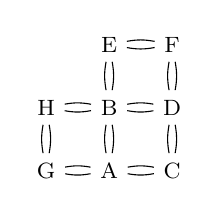
\begin{tikzpicture}[scale=0.8]
        % \tikzstyle{v}=[draw, circle, minimum size=0.1cm, scale=0.7, font=\footnotesize]
        \tikzstyle{v}=[font=\footnotesize]

        \node[v] (a) at (0,0) {A};
        \node[v] (b) at (0,1) {B};
        \node[v] (c) at (1,0) {C};
        \node[v] (d) at (1,1) {D};
        \node[v] (e) at (0,2) {E};
        \node[v] (f) at (1,2) {F};
        \node[v] (g) at (-1,0) {G};
        \node[v] (h) at (-1,1) {H};
    
        \draw (a) to [bend right=10](b);
        \draw (a) to [bend left=10](b);
        \draw (a) to [bend right=10](c);
        \draw (a) to [bend left=10](c);
        \draw (d) to [bend right=10](c);
        \draw (d) to [bend left=10](c);
        \draw (b) to [bend right=10](d);
        \draw (b) to [bend left=10](d);
        \draw (b) to [bend right=10](e);
        \draw (b) to [bend left=10](e);
        \draw (b) to [bend right=10](h);
        \draw (b) to [bend left=10](h);
        \draw (g) to [bend right=10](h);
        \draw (g) to [bend left=10](h);
        \draw (g) to [bend right=10](a);
        \draw (g) to [bend left=10](a);
        \draw (f) to [bend right=10](e);
        \draw (f) to [bend left=10](e);
        \draw (f) to [bend right=10](d);
        \draw (f) to [bend left=10](d);
    \end{tikzpicture}
    \caption{}
\end{subfigure}
\begin{subfigure}{0.3\linewidth}\centering\scriptsize
    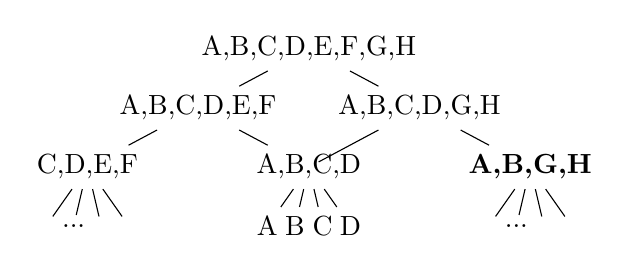
\begin{tikzpicture}
    [level 1/.style={sibling distance=8em},
     level 3/.style={sibling distance=1em}, level distance=0.75cm]
        \tikzstyle{n}=[draw, fill, circle]

        \node (a) at (0,0) {A,B,C,D,E,F,G,H}
            child { node {A,B,C,D,E,F} 
                child { node {C,D,E,F}
                    child {node { }}
                    child {node {...}}
                    child {node { }}
                    child {node { }}
                    } 
                child { node (shared) {A,B,C,D}
                    child {node {A}}
                    child {node {B}}
                    child {node {C}}
                    child {node {D}}
                    } 
                }
            child { node {A,B,C,D,G,H} 
                child { node { } }
                child { node {{\bf A,B,G,H}} 
                    child {node { }}
                    child {node {...}}
                    child {node { }}
                    child {node { }}
                }
            };

    \end{tikzpicture}
    \caption{}
\end{subfigure}
\begin{subfigure}{0.2\linewidth}\centering
    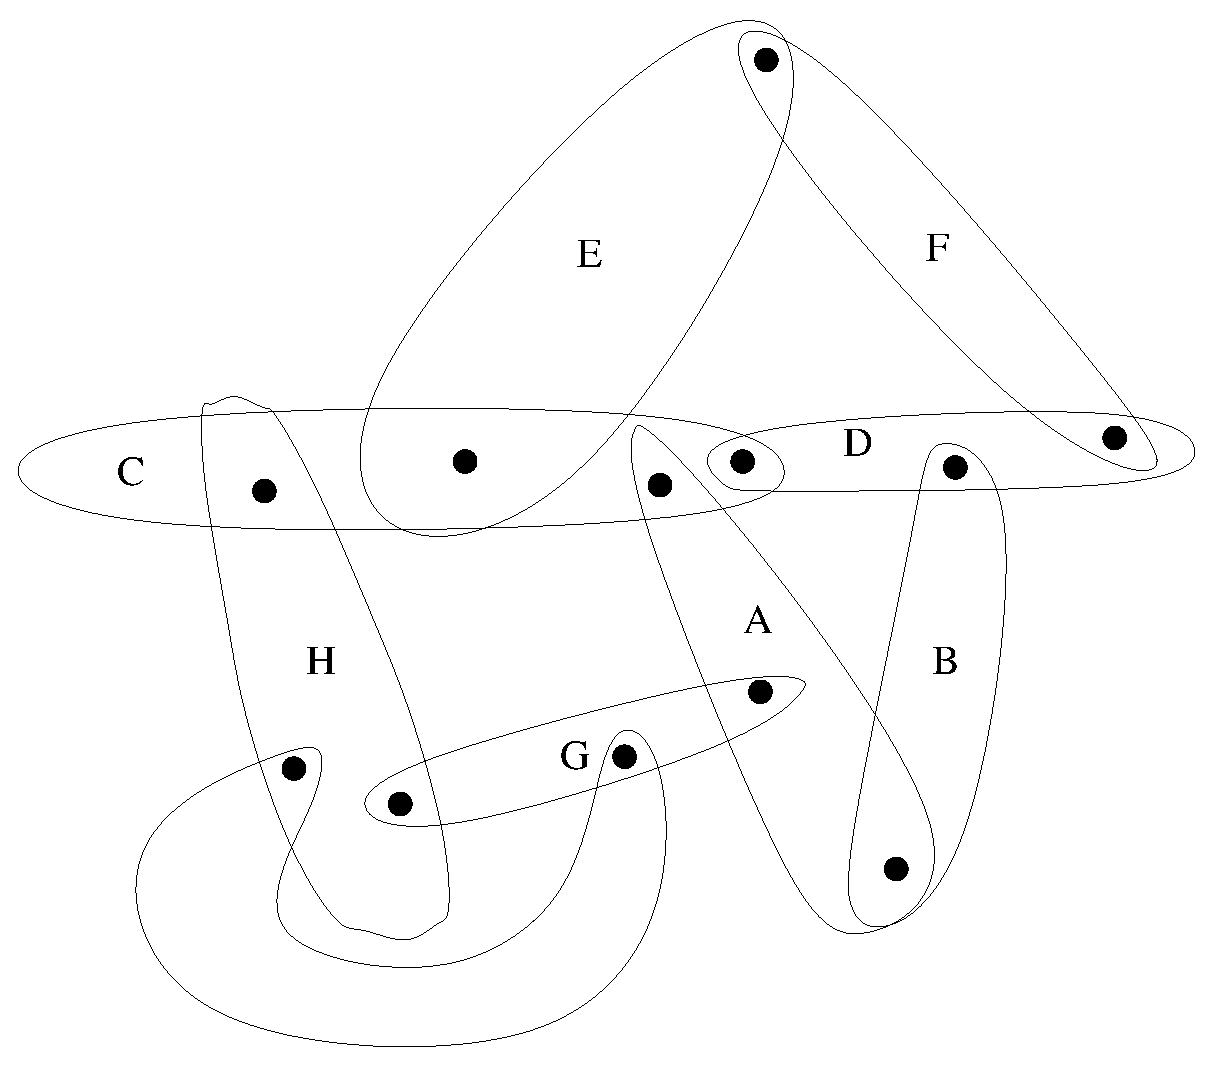
\includegraphics[width=\linewidth]{img/bodypin2}
    \caption{}
\end{subfigure}

% \begin{subfigure}
    
% \end{subfigure}
\caption{(a) is an orignal body-pin qusec. (b) is the corresponding body-bar qusec explained in Definition \ref{def:body-pin}. (c) is the 1 dof DR plan for the qusec. In this case, to obtain an isostatic system, we would need to add a body and 2 pins to one of the node in the second level. (d) is the result of adding one such body tot he bold-faced node.}

\end{figure*}

\begin{theorem}
    There is a quadratic algorithm for the 1 dof and 2 dof optimal completion problem of Seciton \ref{recomb} for body-pin and multi-triangle-pin qusecs.
\end{theorem}

\begin{proof}
    Suppose we are given a body-pin qusec $G$ and have obtained the DR plan denoted $T$. Each node of $T$ will then be a vertex maximal proper 1 dof subgraph of $G$. To make the entire graph wellconstrained, we can add a body and pin it to a node $b$ in $T$ such that the body is pinned to 2 separate children of $b$. From Remark \ref{rem:1dofcanon}, we know that the children can only be joined by a single pin or a single body, so we simply have to pin the new body to one part on each side of the pin or body. Doing so will ensure the following

    \begin{itemize}
        \item All children of $b$ will remain 1 dof
        \item All ancestors of $b$ (including $b$) will now be wellconstrained
    \end{itemize}

    Then, we can form a valid isostatic DR plan $T_b$ from $T$. In $T_b$, $b$'s children are now all of the leaf nodes of the subtree rooted at $b$ because no child of $b$ in $T$ is isostatic. Similarly, for any other node $w$ that is an ancestor of $b$, $w$'s children will be the node that leads to $b$, denoted $b'$, along with all of the other leaf nodes in the tree rooted at $w$ excluding $b'$. Then, for any node $b$ that we choose, $T_b$ is a valid DR plan. Thus, if we want to minimize the size of our DR plan, we simply need to take the $b$ that has the $T_b$ of smallest size. Running this algorithm in a brute force fashion is quadratic in the number of bodies of our given body-pin system.

    For the 2 dof case, we can do something very similar, except instead of pinning a single body 2 times to a node, we can pin another body 2 times to a node. These can be the same node, and if it is the same node, we can find a wellconstrained DR plan in quadratic time, we would just be doing the same thing as the 1 dof case.
\end{proof}
